\begin{frame}{Structure}
    \begin{mdframed}[frametitle=Theoretical Background,%
            backgroundcolor=\ColorIntro]
        What does the energy function model?
    \end{mdframed}

    \begin{mdframed}[frametitle=Methods,%
            backgroundcolor=\ColorMethod]
        Implementation of the function.
    \end{mdframed}

    \begin{mdframed}[frametitle=Results,%
            backgroundcolor=\ColorResults]
        Performance Evaluation
    \end{mdframed}

    \begin{mdframed}[frametitle=Discussion,%
            backgroundcolor=\ColorDiscussion]
    \end{mdframed}
\end{frame}

\section{Theoretical Background}

\colorframe{\ColorIntro}{Theoretical Background}

% Atomic Contact Energy models desolation energy
% measure of stability => popping balloon

\begin{frame}{Appetizer}
    \begin{center}
        \includegraphics[width=0.8\textwidth]{baloon.png}
    \end{center}
    \begin{flushright}
        \tiny
        \color{gray}from: \url{http://thejobmouse.com}
    \end{flushright}
\end{frame}

\begin{frame}{The Free Desolation Energy}
    \begin{itemize}[<+->]
        \item Energy needed for transferring atoms from the solvent (water) into
        the protein's interior.
        \item One possible measure of protein stability
        \item The project:
        \begin{itemize}
            \item Implement desolation energy by \cite{Zhang1997}
            \item Evaluate on \emph{CASP11} data
        \end{itemize}
    \end{itemize}
\end{frame}
% 
% Interaction of atoms keep protein stable
\begin{frame}{Atomic Contacts}
    \begin{center}
        \includegraphics[width=0.8\textwidth]{ace.png}
    \end{center}
    \begin{flushright}
        \tiny
        \color{gray}Based on a picture from: \url{http://thejobmouse.com}
    \end{flushright}
\end{frame}
%
% Model based on atomic contact pairs
% valid if <6A
% 10 bonds away
% picture
\begin{frame}{Atomic Contacts Pairs}
    \begin{center}
        \only<1>{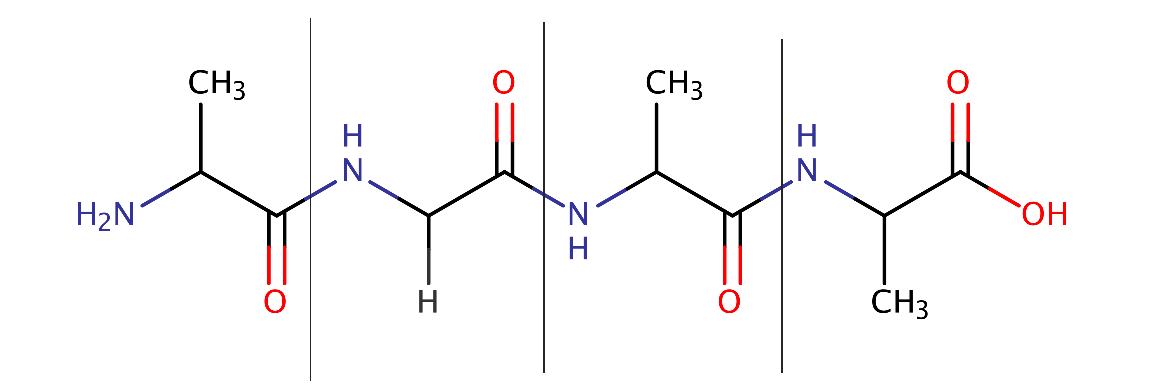
\includegraphics[width=0.8\textwidth]{prot_norm.pdf}}
        \only<2>{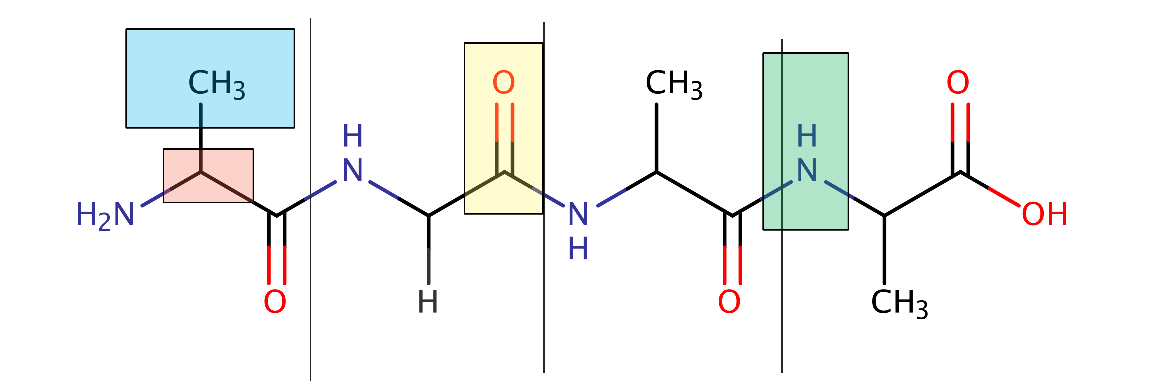
\includegraphics[width=0.8\textwidth]{prot_high.pdf}}
    \end{center}
    A valid contact pair:
    \begin{itemize}
        \item Only heavy atoms
        \item Distance below 6\,\AA
        \item More than 10 covalent bonds in between\\
        \uncover<2->{Estimated by connectivity class \& residue index
        differences}
    \end{itemize}
    Overall energy is a simple sum
\end{frame}
%
% 6A limit from packaging
\begin{frame}{Atomic Packaging}
    \begin{center}
        \includegraphics[width=0.9\textwidth]{../results/Density/better.pdf}
    \end{center}

    \begin{itemize}
        \item Number density of interior atoms (SAS = 0)
        \item Relative to a sphere of variable radius
        \item Evaluated on non-homologous protein set
    \end{itemize}
\end{frame}

